Daiet \cite{daiet} is a system that performs in-network data aggregation for partition/aggregate data center applications (big data analysis such as MapReduce \cite{mapreduce}, machine learning, graph processing and stream processing).
Instead of letting worker servers entirely perform computation on the data and then communicate with each other to update shared state or finalize the computation, the system let network devices perform data aggregation in order to achieve traffic reduction, thus reducing the processing load at the destination.\par
The inventors have proven that in-network data aggregation can reduce the network traffic significantly for machine learning algorithms (e.g., TensorFlow \cite{tensorflow}) and for graph analytics algorithms (e.g., GPS \cite{gps}), hence justifying the usefulness of this system. The system has been designed for P4 \cite{p4} and programmable ASICs, and it can be used on any other \gls{sdn} platform.

\subsubsection{Details}
\paragraph{Controller}
When executing a MapReduce program, the job allocator informs the network controller of the job allocation to the workers.
Then, the network controller pushes a set of rules to network devices in order to
\begin{mylist}
    \item establish one aggregation tree for each reducer and
    \item perform per-tree aggregation
\end{mylist}.
An aggregation tree is a spanning tree from all the mappers to the reducer.

\begin{figure}[!htb]
    \centering
        % trim = left, bottom, right, top
        \includegraphics[page=9, clip, trim=0.25cm 1.1cm 0.25cm 4.7cm, width=1.00\textwidth]{figures/analysis/inp/solutions.pdf}
    \caption{Daiet's \texorpdfstring{\cite{daiet}}{} basic topology and entities}
\end{figure}

\paragraph{Packets}
Since every reducer has its own aggregation tree associated with it, network devices should know how to correctly forward traffic according to the corresponding tree: to achieve this, a special \textit{tree ID} (that could coincide with the \textit{reducer ID}) packet field allows network devices to distinguish different packets belonging to different aggregation trees.

\begin{figure}[!htb]
    \centering
        % trim = left, bottom, right, top
        \includegraphics[page=10, clip, trim=0.5cm 0.7cm 1.2cm 2.7cm, width=1.00\textwidth]{figures/analysis/inp/solutions.pdf}
    \caption{Daiet's \texorpdfstring{\cite{daiet}}{} extended topology}
\end{figure}

Obviously, they must also know the output port towards the next network device in the tree and the aggregation function to be performed on the data.

\begin{figure}[!htb]
    \centering
        % trim = left, bottom, right, top
        \includegraphics[page=11, clip, trim=0.35cm 0.6cm 0.3cm 2.7cm, width=1.00\textwidth]{figures/analysis/inp/solutions.pdf}
    \caption{Daiet's \texorpdfstring{\cite{daiet}}{} logical communication pattern}
\end{figure}

Packets are sent via UDP (therefore communication is not reliable) with a small preamble that specifies
\begin{mylist}
    \item the number of key-value pairs contained in the packet and
    \item the \textit{tree ID} whose packet belongs to
\end{mylist}.
They payload is not serialized to achieve a faster computation by network devices.

\subsubsection{Algorithm} \label{daiet_algorithm}
To store the key-value map, network devices use two hash tables for each tree: one for the keys and one for the values.
Upon a collision, the algorithm checks whether the key is matching or just the hash is.
In the former case, data aggregation is performed.
In the latter case, the conflicting pair will end up in a \textit{spillover bucket} that will be flushed to the next node as soon as it becomes full: this is done since this data is more likely to be aggregated by the next network device if it has spare memory.

\begin{figure}[!htb]
    \centering
        % trim = left, bottom, right, top
        \includegraphics[page=12, clip, trim=2.1cm 0.3cm 2cm 0.25cm, width=1.00\textwidth]{figures/analysis/inp/solutions.pdf}
    \caption{Messages exchanged during a Daiet \texorpdfstring{\cite{daiet}}{} instance execution}
\end{figure}

A network device will also flush its data as soon as all its children (according to the aggregation tree) have sent their data: this is made possible by forcing network devices to send a special \textit{END} packet after transmitting all key-value pairs to their successor.\par
Used indexes are stored in a \textit{index stack} to avoid scanning the whole hash table when flushing.

\subsubsection{Implementation} \label{daiet_implementation} \label{p4_drawbacks}
The network data plane has been programmed using P4 \cite{p4}, which brings two main drawbacks:
\begin{mylist}
    \item a match-action table cannot be applied more than once for the same packet, forcing the programmer to perform loop unrolling in case of multiple headers in the same packet that need to be modified by the same rule table and
    \item keys must have a fixed size, causing a big waste of memory in applications where keys have variable-lengths (e.g., strings)
\end{mylist}.
The second drawback will also cause arrays to have fewer but bigger cells, thus increasing the probability of collisions.
If these collisions involve pairs having different keys (\cref{daiet_algorithm}), data will not be aggregated, causing traffic to increase.

\subsubsection{Minimum system requirements}
For each aggregation tree (i.e., for each reducer), network devices must form a tree whose root is connected to the reducer and whose leaves are connected to mappers.
Each mapper has to be connected to exactly one network device of the lowest level.
Network devices must
\begin{mylist}
    \item store two arrays (one for the keys and one for the values) and
    \item be able to hash keys
\end{mylist}.
The solution requires that the system has a centralized \gls{sdn} controller connected to all switches.
The \gls{sdn} controller must push flow rules to all switches belonging to at least one tree.

\subsubsection{Conclusions}
Besides all the drawbacks brought by P4 \cite{p4} listed in \cref{daiet_implementation}, inventors claim to achieve a 86.9\%-89.3\% traffic reduction, causing the execution time at the reducer to drop by 83.6\% on average.